% =====================================================================
%  Capítulo 8 — Resultados
%  Versão AP2: o placar e a discussão da AP1 ficam como ponto de partida
%  e devem ser atualizados com os resultados da campanha.
% =====================================================================
\chapter{Resultados}
\label{cap:resultados}
\rubricaComunicacao

\begin{orientacao}
Resultado é número com procedência, não adjetivo. Cada afirmação deste
capítulo deve poder ser rastreada até um caso de teste do
Capítulo~\ref{cap:testes} ou até uma tabela dos apêndices.
Um gráfico bem escolhido resolve mais do que uma página de texto ---
e um gráfico sem unidade no eixo não resolve nada.

Na AP2, o gráfico principal é a \textbf{série temporal da campanha},
com as lacunas visíveis: não interpolem para o gráfico ficar bonito.
Marquem no gráfico os disparos do alarme e os eventos do registro do
Apêndice~\ref{ap:campanha}, se houver.
\end{orientacao}

\section{O sistema em operação}

\begin{figure}[H]
\centering
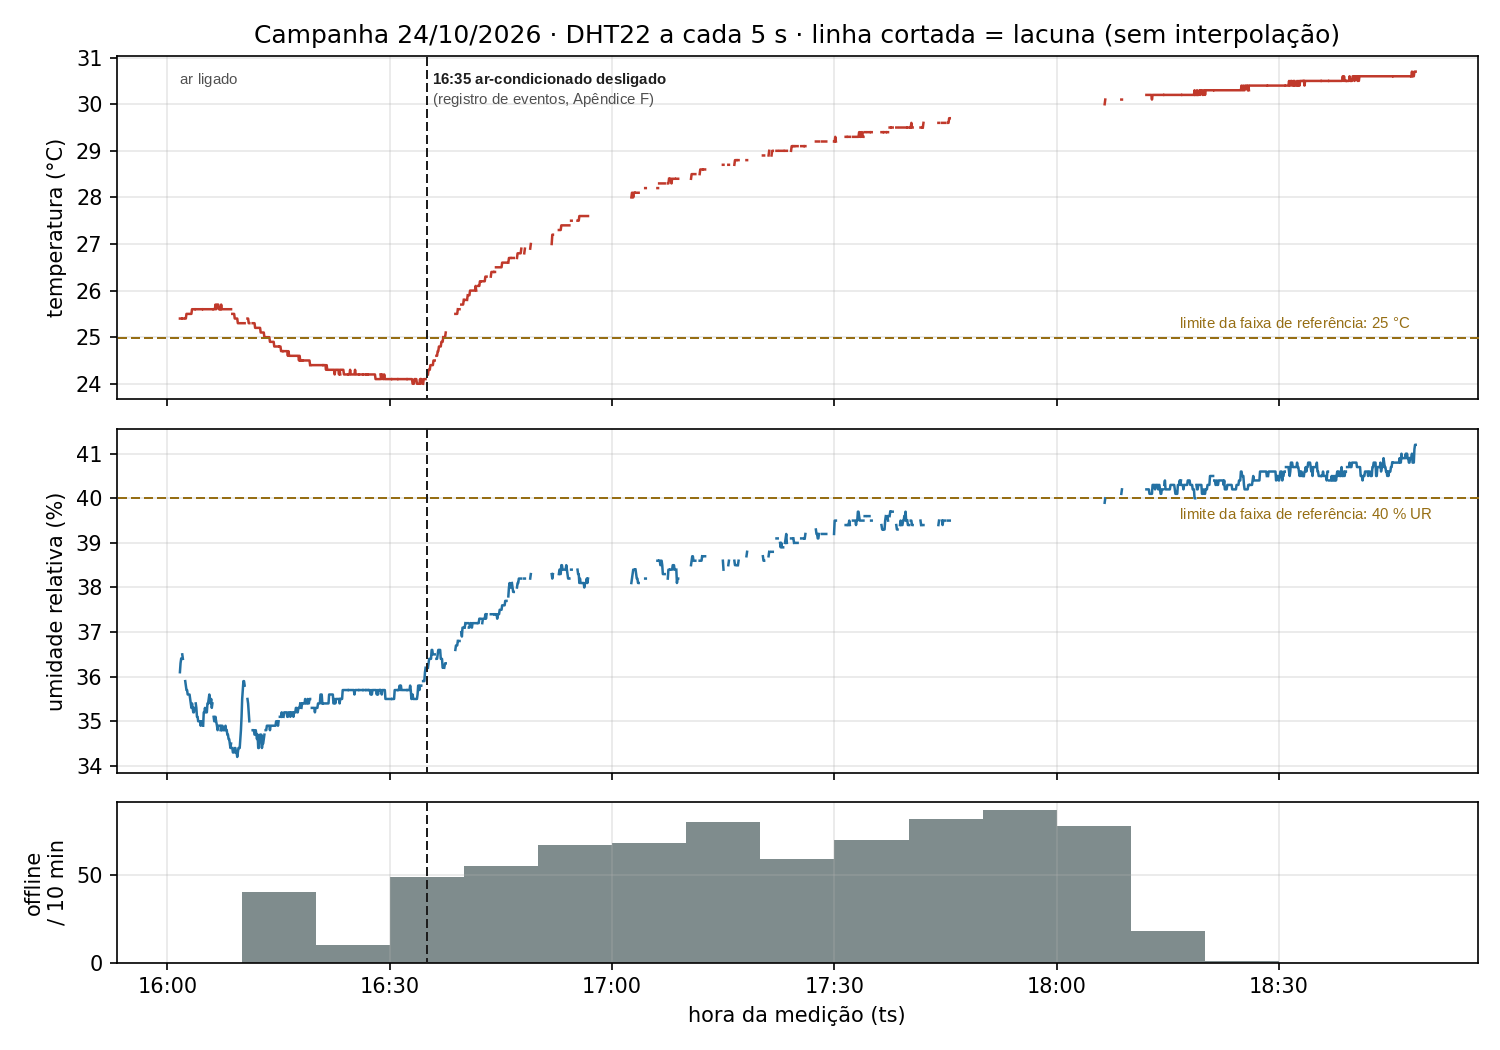
\includegraphics[width=0.95\textwidth]{figuras/serie-campanha-anotada.png}
\caption{Série temporal da campanha de coleta: temperatura, umidade
  relativa e quedas de conexão (\texttt{offline} a cada
  \SI{10}{\minute}), com o evento do registro (16:35) e os limites da
  faixa de referência. A linha é cortada onde falta leitura; nada foi
  interpolado}
\label{fig:resultado}
\fonte{Dados coletados pela equipe em 24/10/2026, das 16:01 às 18:48
  (\texttt{dados/campanha\_24-10-26/mensagens.csv}, branch
  \texttt{lab3}); gráfico gerado por \texttt{gravador/grafico.py}. As
  barras de \texttt{offline} usam a hora de chegada ao gravador; a de
  16:10 inclui os testamentos de 16:01 a 16:10, que chegaram no lote
  guardado pelo \emph{broker}. A linha do evento e as da faixa de
  referência foram acrescentadas pela equipe sobre a saída do
  \texttt{grafico.py}, que está sem anotações em
  \texttt{dados/campanha\_24-10-26/serie\_temporal.png}.}
\end{figure}

A série mostra um único evento, e ele está anotado: o ar-condicionado
do cômodo foi desligado às 16:35 (Apêndice~\ref{ap:campanha}). Com o ar
ligado, a temperatura caiu devagar, de 25,7 para \SI{24,0}{\celsius}.
Desligado o aparelho, ela subiu cerca de \SI{2}{\celsius} em
\SI{6}{\minute} (\SI{24,0}{\celsius} pouco antes, \SI{24,2}{\celsius} às
16:35 e \SI{26,0}{\celsius} às 16:41) e
continuou subindo, cada vez mais devagar, até \SI{30,7}{\celsius} no
fim, sem estabilizar. A curva é contínua mesmo durante a fase degradada
da conexão: as lacunas tiram pontos da série, mas não mudam a forma
dela. A umidade relativa subiu junto, de 34 para 41\,\%. Só o
aquecimento faria a umidade relativa cair; uma explicação compatível é
que o ar-condicionado, ligado, condensa e retira vapor do ar, e
desligado deixa de retirar. É uma hipótese: a umidade absoluta não foi
medida.

O alarme não aparece no gráfico porque o \emph{firmware} da campanha não
tem alarme (Seção~\ref{sec:firmware-com}). Aplicada depois, sobre o CSV,
a faixa padrão do \emph{firmware} da AP1 (a da sala de manipulação: 15
a \SI{25}{\celsius} e 40 a 70\,\% UR, Tabela~\ref{tab:config}) mostra
que o cômodo \textbf{nunca esteve dentro dela}: a temperatura só ficou
abaixo de \SI{25}{\celsius} entre 16:13 e 16:37, com o ar ligado, e ficou
acima dela em todas as 821 leituras depois das 16:37 (944 das \num{1213}
leituras com o DHT22, no total); a umidade ficou abaixo de 40\,\% UR até as 18:06 (778
leituras). Com a regra da Listagem~\ref{lst:alarme}, o nó da AP1 teria
pulsado o alarme a cada minuto durante toda a tarde. Não é defeito do
cômodo: a faixa é a de uma sala controlada, e um quarto em Teresina, de
tarde, não é uma; por isso a faixa é configurável por ambiente
(\RF{02}).

As lacunas estão na Tabela~\ref{tab:lacunas} e na barra de baixo da
Figura~\ref{fig:resultado}. Todas coincidem com quedas de conexão
registradas no \texttt{status}: o nó não reiniciou sozinho, o gravador
não parou, e não houve falta de energia. A maior parte delas está entre
16:30 e 18:10, a fase em que o nó conectava e caía em ciclo
(Seção~\ref{sec:qualidade}).

\section{Requisitos atendidos}

\begin{orientacao}
Retome a Tabela~\ref{tab:rastreabilidade} e feche o placar: quantos
requisitos foram atendidos, quantos parcialmente, quantos não. Para cada
não atendido, uma frase dizendo o que faltou. Equipe que declara
honestamente dois requisitos não atendidos sai melhor do que equipe que
declara todos atendidos e é desmentida na demonstração.
\end{orientacao}

\textbf{Ponto de partida (AP1).} Dos 9 requisitos definidos no primeiro
ciclo, a AP1 declarou 2 atendidos (\RF{01} e \RNF{03}), 4 parciais
(\RF{02}, \RF{03}, \RF{04} e \RNF{01}) e 3 não verificados ou não
atendidos (\RNF{02}, com latência observada de $\approx$\SI{5}{\second}
contra a meta de \SI{2}{\second}; \RNF{04} e \RNF{05}, não testados). As
pendências eram: o ensaio de alteração de faixa (\RF{02}), a latência do
alarme (\RNF{02}), o log formal da cessação do alarme (\RF{04}), a
medição de autonomia com bateria real (\RNF{01}) e os ensaios de faixa de
operação e de interferência (\RNF{04} e \RNF{05}). O \RF{01} continua
atendido, agora com a conta explícita: o \CT{01} rodou em modo
acelerado, mas dele se deduz a parte ativa do ciclo ($\approx$\SI{8,7}{\second}),
e com o sono de \SI{600}{\second} o ciclo fica 1,5\,\% acima de
\SI{10}{\minute}, dentro da tolerância.

\textbf{Placar da AP2.} Com os 7 requisitos de comunicação e de dados
acrescentados neste ciclo (\RF{05} a \RF{08} e \RNF{06} a \RNF{08}), o
sistema tem 16 requisitos: \textbf{5 atendidos} (\RF{01}, \RF{05},
\RF{07}, \RNF{03} e \RNF{06}), \textbf{8 parciais} (\RF{02}, \RF{03},
\RF{04}, \RF{06}, \RF{08}, \RNF{01}, \RNF{05} e \RNF{08}) e \textbf{3
não atendidos ou não testados} (\RNF{02}, \RNF{04} e \RNF{07}). Dos
cinco atendidos, dois se apoiam em estimativa declarada: o \RF{01}
(intervalo extrapolado do \CT{01}) e o \RF{07} (atraso do testamento
descontado o trânsito até o gravador). Os que não foram atendidos:

\begin{itemize}
  \item \RNF{07}: a completude foi de 63,1\,\%, contra a meta de
    95\,\%. As fases estáveis ficaram em 96\,\%, no limite da meta; a
    fase degradada, de \SI{1}{\hour} e \SI{40}{\minute}, derrubou a
    média. Faltou fila local, que teria guardado as leituras das quedas
    curtas, e faltou confirmar a causa das quedas;
  \item \RNF{02} e \RNF{04}: continuam como na AP1. O \emph{firmware}
    da campanha não tem alarme, e nenhum dos dois foi refeito.
\end{itemize}

\noindent Os parciais ficaram assim por motivos concretos: o \RF{06}
reconecta sozinho (nas 553 quedas do \emph{broker} da campanha, em
\SI{3,5}{\second} na mediana e em até \SI{30}{\second} em 552 delas),
mas não guarda; o \RF{08} não tem o \texttt{boot}; o \RNF{08} foi verificado até
\SI{8,7}{\minute}, e não até os \SI{10}{\minute} da meta; o \RNF{01}
chega a $\approx$29 dias só com o nó central e LoRa (estimativa de
folha de dados, sem o módulo), e o nó que publica direto ao roteador
fica em 21 dias, o número que leva o produto a ter um nó central
(\DP{6} e \DP{8}). O \RNF{05} passou de \enquote{não testado} a parcial com os
33 minutos de ar-condicionado ligado da campanha. Das pendências da AP1,
nenhuma foi resolvida neste ciclo: o trabalho foi
para a comunicação, que rodou num \emph{firmware} separado.

\section{Discussão}

\begin{orientacao}
Cinco perguntas, uma resposta curta para cada. As três primeiras vêm da
AP1 e continuam valendo; as duas últimas são da AP2.
\end{orientacao}

\begin{enumerate}[label=\arabic*.]
  \item \textbf{O sistema responde à pergunta de projeto do
    Capítulo~\ref{cap:problema}?} Na AP1, a resposta cobria apenas a
    metade local da pergunta: captar temperatura e umidade e sinalizar
    no ambiente quando saem da faixa. Na AP2, as leituras passaram a
    chegar a um ponto central, o gravador, com \SI{0,8}{\second} de
    atraso mediano, e um nó morto aparece no \texttt{status} em
    \SI{46}{\second}. Levadas pela ponte ao servidor do produto, as
    \num{1213} leituras da campanha entraram no banco e no painel sem
    nenhuma rejeitada (\CT{16}): o caminho até o servidor central da
    pergunta de projeto foi exercitado de ponta a ponta com dado real,
    ainda sem o nó central em hardware. Mas as duas metades ainda não estão no mesmo nó: o
    \emph{firmware} que publica não tem o alarme, e o que tem o alarme
    não publica. E, numa tarde, 37\,\% das leituras não chegaram: a
    condição da sala passou a ser conhecida sem ronda nos trechos
    estáveis, e não durante a fase degradada.
  \item \textbf{Qual decisão de projeto se mostrou mais acertada, e qual
    a equipe refaria?} Na AP1, a equipe apontou o processamento dos dados
    agregados fora do nó (\DP{5}), pelo custo energético de qualquer
    processamento extra na borda, e não identificou decisão a refazer.
    Na AP2, a mais acertada foi guardar o dado num assinante com sessão
    persistente (\DP{7}): o gravador começou \SI{8,7}{\minute} atrasado e
    não perdeu nenhuma leitura por isso. A que a equipe refaria é
    publicar só quando há conexão, sem fila: foi ela que transformou cada
    queda de conexão em leitura perdida. O \emph{deep sleep} da \DP{4}
    não chegou à campanha: o nó ficou sempre conectado e na USB
    (\DP{6}).
  \item \textbf{Se a autonomia real for metade da calculada, o projeto
    ainda faz sentido?} Na AP1, a equipe respondeu que uma autonomia pela
    metade tornaria a manutenção mais frequente do que o modelo de
    negócio pretende, em ambientes de acesso restrito. Com o rádio
    medido, a autonomia calculada do nó que publica direto ao roteador é
    de 21 dias; a metade seria cerca de 10 dias, uma troca de bateria a
    cada semana e meia, o que não faz sentido para o produto. Por isso o
    produto passa a ter um nó central (\DP{6} e \DP{8}): com LoRa, o
    rádio do nó de borda deve custar 2 a \SI{3}{\mAh}/dia
    (\folhadedados), a autonomia fica em $\approx$29 dias, e a metade
    dela, perto dos 15 dias, ainda é o dobro da do WiFi direto. O número
    só será confirmado quando o módulo LoRa chegar.
  \item \textbf{A tecnologia escolhida se sustentou?} O WiFi, sim: com
    RSSI entre \SI{-15}{} e \SI{-29}{dBm}, o enlace de rádio não foi o
    problema. O que não se sustentou foi a conexão MQTT ao \emph{broker}
    público: 764 quedas em \SI{2,78}{\hour} e completude de 63,1\,\%,
    contra cerca de 96\,\% nos trechos estáveis. O WiFi deixaria de
    servir com o nó a mais de duas paredes ou \SI{11}{\metre} do
    roteador, ou dentro de uma câmara metálica (\DP{8}).
  \item \textbf{O conjunto de dados responde ao que a equipe quer fazer
    na AP3?} Ainda não. Ele tem um único exemplo do evento de interesse,
    o ar-condicionado desligado às 16:35, numa só tarde, num cômodo e
    não no cenário de referência. Serve para escolher a janela e as
    características (a taxa de subida da temperatura e a umidade
    subindo junto); para treinar e validar, faltam mais eventos
    anotados (Seção~\ref{sec:dataset}).
\end{enumerate}
